\documentclass[__main__.tex]{subfiles}

\begin{document}

\qtitle{О}{01}
Принцип Гюйгенса-Френеля. Метод зон Френеля. Классификация дифракционных явлений.\\ 

%%
\textbf{Принцип Гюйгенса-Френеля. }\\

\begin{figure}[h]
	\begin{center}
		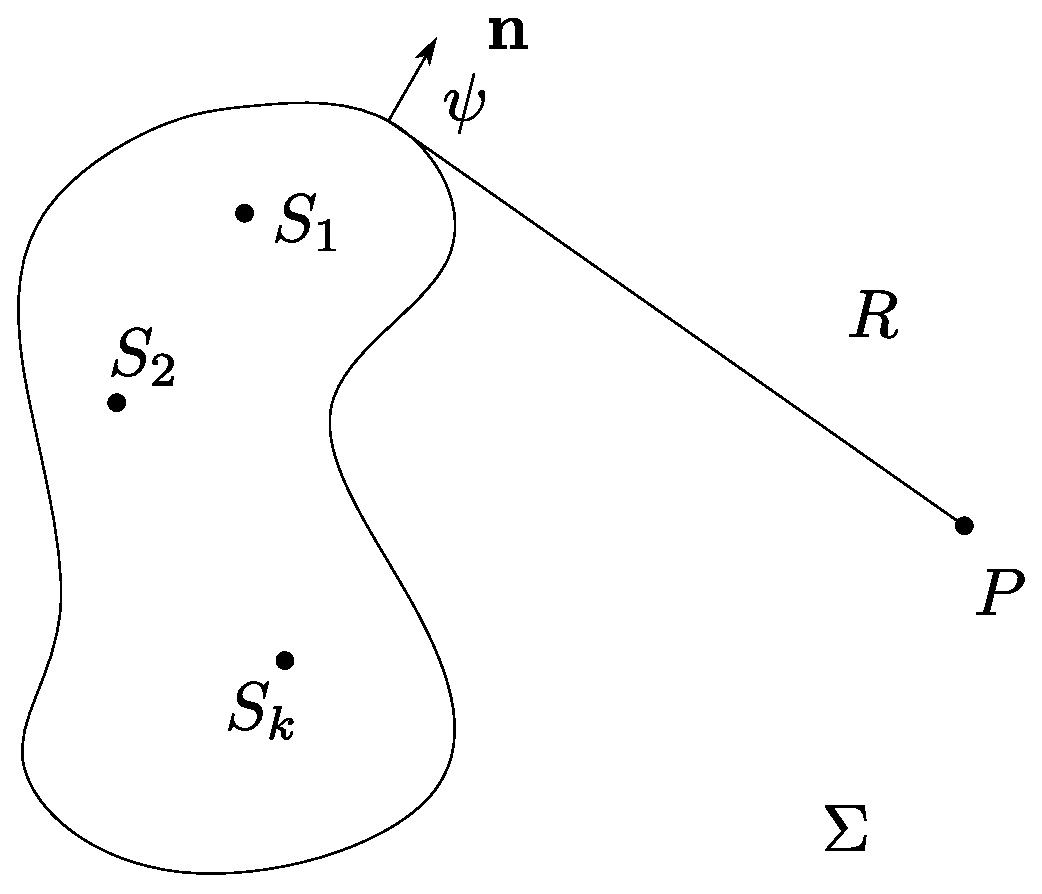
\includegraphics[width=0.5\linewidth]{o-08_1.eps}
	\end{center}
\end{figure}
\begin{enumerate}
\item
Если окружить систему когерентных источников произвольной замкнутой поверхностью $\Sigma$, то каждую точку этой поверхности можно считать источником вторичных когерентных сферических волн, распространяющихся по всем направлениям. Амплитуда этих волн на поверхности находится как суперпозиция волн, идущих от первичных источников. Световое поле в любой точке вне этой поверхности можно рассчитывать как суперпозицию всех вторичных волн;
\item
Если часть этой поверхности закрыта непрозрачным экраном, то учитывать нужно только волны, идущие от открытых частей поверхности.
\end{enumerate}
Обе эти части принципа объединяет дифракционный интеграл Релея:
$$E(P) = \frac{1}{i\lambda}\iint\limits_{\Sigma'} \widetilde K(\psi) E(Q)\frac{e^{ikR}}{R}d\sigma,$$
где $\Sigma'$ - открытая часть поверхности $\Sigma$, $Q$ - точка на $\Sigma'$, $E(Q)\frac{e^{ikR}}{R}$ - сферическая волна, идущая от этой точки 


\textbf{Метод зон Френеля}\\

\begin{figure}[h]
	\begin{center}
		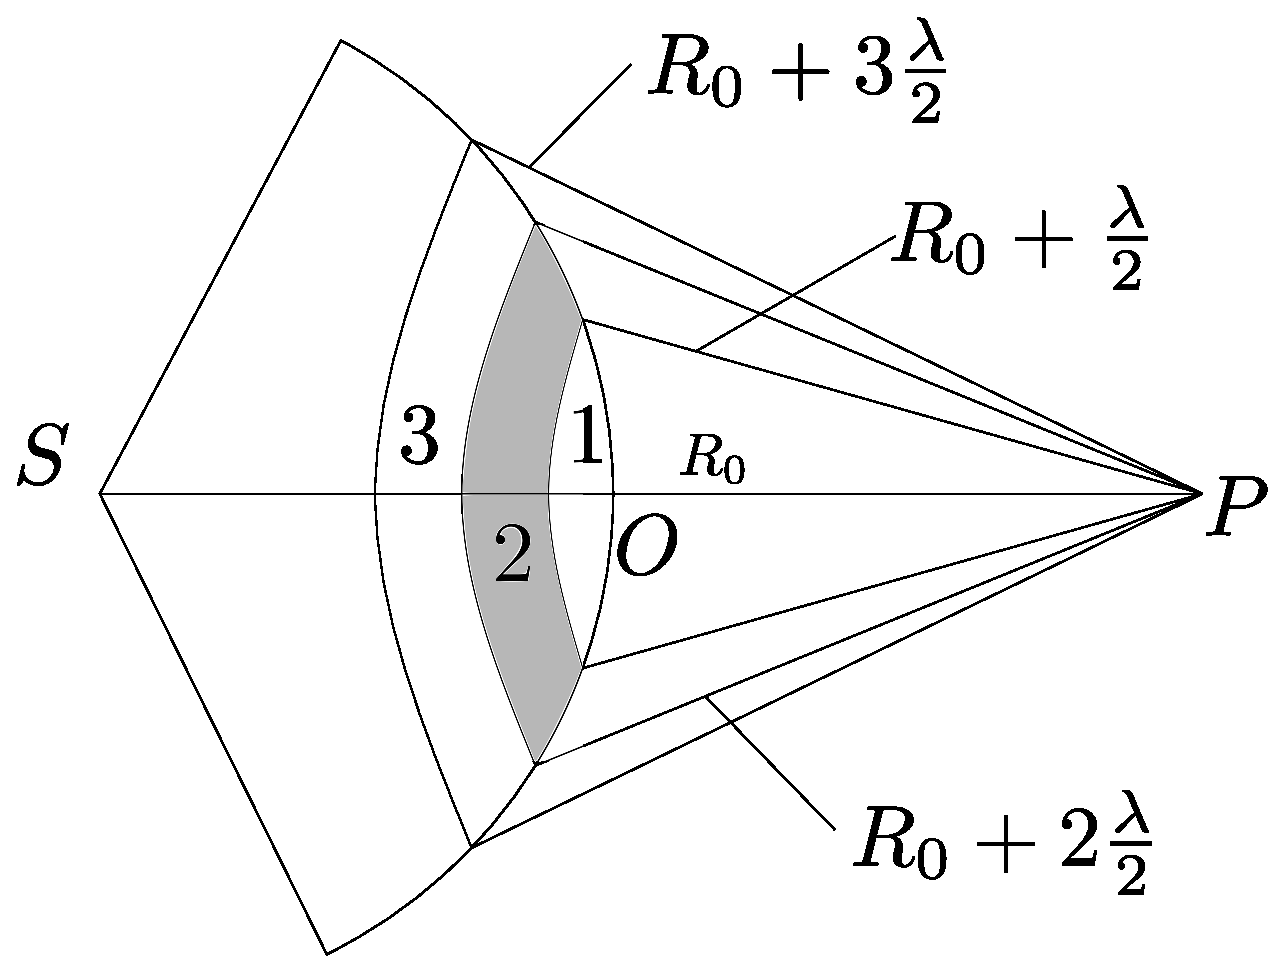
\includegraphics[width=0.5\linewidth]{o-08_2.eps}
	\end{center}
\end{figure}

Суть наблюдаемого эффекта заключается в том, что при изменении в определенных пределах радиуса диафрагмы в точке $P$ наблюдается то светлое, то темное пятно. Для объяснения этого эффекта Френель предложил разбить вспомогательную поверхность на зоны. Первая зона Френеля представляет собой шапочку на сфере, граница которой отстоит от точки $P$ на расстояние $R_1 = R_0 + \frac{\lambda}{2}$, так что ей принадлежат все точки сферы в пределах $R_0 < R < R_0 + \frac{\lambda}{2}$. Все остальные зоны - пояса. Вторая зона задается условиями $R_0 + \frac{\lambda}{2} < R < R_0 + \frac{2\lambda}{2}$, ее внешняя граница удалена от точки наблюдения на расстояние $R_2 = R_0 + \frac{2\lambda}{2}$. Для $m$-той зоны:
$$R_{m-1} < R < R_m,$$
$$R_m = R_{m-1} + \frac{\lambda}{2} = R_0 + m\frac{\lambda}{2}$$
Используем формулу
$$E = E_0\left(K(R_{min}) e^{ik(R_{min} - R_0)} - K(R_{max})e^{ik(R_{max} - R_0)} \right)$$
В случае, если диафрагма открывает первую зону Френеля:
\begin{gather*}
R_{min} = R_0, \qquad R_{max} = R_0 + \frac{\lambda}{2} , \\
e^{ik(R_{min} - R_0)} = 1, \qquad e^{ik(R_{max} - R_0)} = e^{ik\frac{\lambda}{2}} = e^{i\pi} = -1
\end{gather*}
Поле от первой зоны Френеля:
$$E^{(1)} = E_0(1 + K(R_1))$$
Аналогичные расчеты дадут для второй зоны Френеля:
$$E^{(1)} = - E_0(K(R_1) + K(R_2))$$
Для $m$ - той зоны:
\begin{gather*}
R_{min} = R_0 + (m - 1)\frac{\lambda}{2}, \qquad R_{max} = R_0 + m\lambda \\
e^{ik(R_{min} - R_0)} = e^{\frac{i(m-1)k\lambda}{2}} = e^{i(m-1)\pi} = (-1)^{m-1}, \qquad 
e^{ik(R_{max} - R_0)} = e^{ikm\frac{\lambda}{2}} = e^{im\pi} = (-1)^m\\
E^{(m)} = E_0\left((-1)^{m-1} K(R_{m-1}) - (-1)^m K(R_m)\right) = E_0(-1)^{m-1} (K(R_{m-1}) + K(R_m))
\end{gather*} 

\textbf{Классификация дифракционных явлений}\\

Если диафрагма закрыта, то понятно, что за ней нет никакой волны. Будем постепенно ее открывать. В точке наблюдения будет монотонно расти освещенность. В этой области ($m << 1$) на оси ничего интересного не происходит, но на экране наблюдаются кольца – дифракция уже есть и в этих условиях, она называется дифракцией Фраунгофера.
Мы уже устремили источник в бесконечность. Если $m << 1$,
то и точка наблюдения очень далеко ($b \rightarrow \infty$). На диафрагму падает почти параллельный пучок света, и за диафрагмой распространяются лучи параллельные лучи в различных направлениях. Поэтому дифракцию Фраунгофера еще называют дифракцией в параллельных лучах.\\
Так будет продолжаться до тех пор, пока число $m$ не станет равным единице – это максимум, соответствующий одной открытой зоне Френеля. Далее последует минимум с почти нулевой интенсивностью (две открытые зоны), и затем максимумы, уменьшаясь по интенсивности, будут чередоваться с минимумами, которые все больше и больше будут отличаться от нуля. Дифракция в условиях, когда число $m$ равняется нескольким единицам, называется дифракцией Френеля.
Наконец, при дальнейшем увеличении радиуса диафрагмы интенсивность становится равной интенсивности в отсутствие преград, лучи распространяются прямолинейно, так что при $m >> 1$ мы переходим в область геометрической
оптики.\\
\end{document}